\documentclass{beamer}
\usepackage{beamerthemeshadow}
\usepackage{verbatim}

\usepackage{lastpage}
\usepackage{xcolor}
\usepackage{pgf}
\usepackage{colortbl}
\usepackage{hyperref}
\usepackage{multirow}
\usepackage{dsfont}
\usepackage{graphbox}


\usepackage{siunitx}
\sisetup{input-symbols=(), group-digits  = false} 

\newcommand{\bi}{\begin{itemize}}
\newcommand{\ei}{\end{itemize}}
\newcommand{\be}{\begin{enumerate}}
\newcommand{\ee}{\end{enumerate}}
\newcommand{\bd}{\begin{description}}
\newcommand{\ed}{\end{description}}
\newcommand{\prbf}[1]{\textbf{#1}}
\newcommand{\prit}[1]{\textit{#1}}
\newcommand{\beq}{\begin{equation}}
\newcommand{\eeq}{\end{equation}}
\newcommand{\bdm}{\begin{displaymath}}
\newcommand{\edm}{\end{displaymath}}

\newcommand{\ft}[1]{
  \frametitle{\begin{tabular}{p{4.2in}r} \textcolor{white}{#1} & \small{\insertframenumber / \inserttotalframenumber} \end{tabular}}
  \setbeamercovered{transparent=18}
}

\newcommand{\eft}[1]{
  \frametitle{\begin{tabular}{p{4in}r} \textcolor{white}{#1} & \small{\hyperlink{f:questions}{\beamergotobutton{GO BACK}}} \end{tabular}}
  \setbeamercovered{transparent=18}
}

\newcommand{\stepinv}{\setbeamercovered{invisible}}
\newcommand{\stopinv}{\setbeamercovered{transparent=18}}
\newcommand{\uncoverinv}[1]
{
  \setbeamercovered{invisible}
  \uncover<+->{#1}
  \setbeamercovered{transparent=18}
}
\newcommand{\ans}[1]{\textcolor{blue}{#1}}
\newcommand{\ansinv}[1]
{
  \setbeamercovered{invisible}
  \uncover<+->{\textcolor{blue}{#1}}
  \setbeamercovered{transparent=18}
}
\newcommand{\setinv}{\setbeamercovered{invisible}}
\newcommand{\setvis}{\setbeamercovered{transparent=18}}
\newcommand{\centerpic}[2]
{
  \begin{center}
  \includegraphics[#1]{#2}
  \end{center}
}
\newcommand{\h}[1]{\hat{#1}}
\newcommand{\ds}{\displaystyle}

\definecolor{light}{rgb}{1.0,0.7,0.7}
\definecolor{BrickRed}{rgb}{0.8,0.1,0.1}
%\definecolor{light}{rgb}{1.0,0.5,0.5}
%\newcommand{\hl}[1]{\only<#1>{\cellcolor{BrickRed}}}
\newcommand{\hl}[1]{\textcolor<#1>{BrickRed}}

\definecolor{mycolor}{rgb}{0.6,0.0,0.0}
\usecolortheme[named=mycolor]{structure}

\title[Regime Switching in Fiscal Policy in the United States]{Regime Switching in Fiscal Debt Targets and Policy Functions in the United States}
\author[James M. Murray, Dept. of Economics]
{
James M. Murray, Ph.D.\\
Department of Economics
}
\date{January 19, 2018}

\begin{document}

\frame{\titlepage \setcounter{framenumber}{0}}

\begin{frame}
  \ft{What is Fiscal Policy?}

  \uncover<+->{
    \begin{block}{Fiscal Policy}
      Government budget decisions that target...
      \begin{enumerate}
      \item macroeconomic objectives or...
      \item levels of \textit{long-run government debt}.
      \end{enumerate}
    \end{block}
  }
  
  \uncover<+->{
    \begin{block}{Macroeconomic Objectives}
      \begin{itemize}
      \item \textit{Unemployment rate:} Percentage of all those willing and able to work who do not have employment
      \item \textit{Real GDP:} Measure of the total quantity of economic activity in a country a given year
      \item \textit{Output gap:} Percentage difference between real GDP and \textit{potential GDP} \textbf{(Focus)}
      \end{itemize}
    \end{block}
  }
  
\end{frame}

\begin{frame}
  \ft{Macroeconomic Objectives}
  \begin{columns}
    \begin{column}{0.5\textwidth}
      \ \ \ \ \ Unemployment Rate
      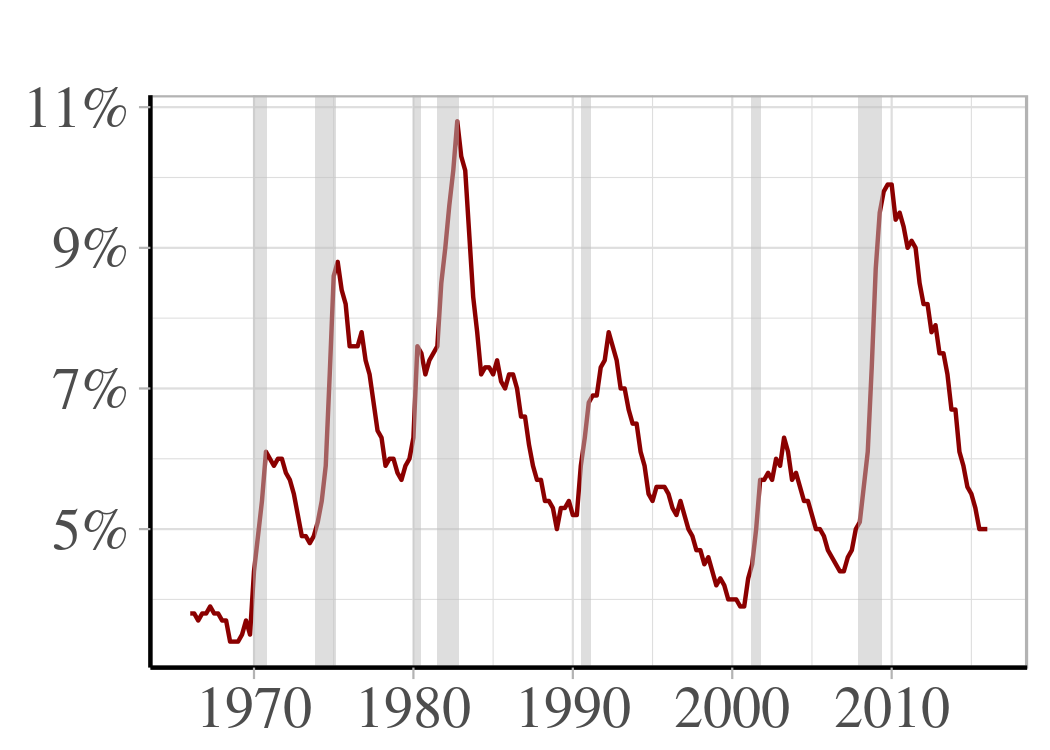
\includegraphics[width=\textwidth]{./plots/unemployment.png}
    \end{column}

    \begin{column}{0.5\textwidth}
      \ \ \ \ \ Output Gap
      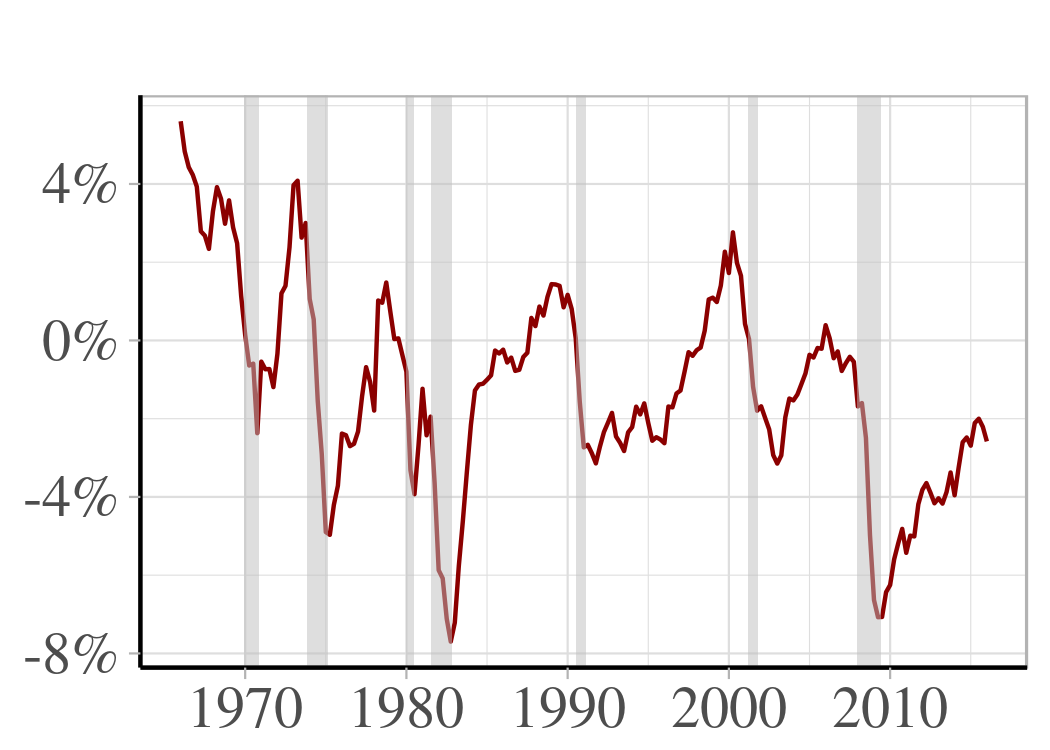
\includegraphics[width=\textwidth]{./plots/outputgap.png}
    \end{column}
  \end{columns}
\end{frame}

  
\begin{frame}
  \ft{Debts and Deficits}
  
  \uncover<+->{\begin{block}{Federal government debt}
    Total value of all outstanding funds borrowed by the federal government that are outstanding.
    \begin{itemize}
    \item \textit{Stock variable}
    \end{itemize}
  \end{block}}
    
  \uncover<+->{\begin{block}{Federal government deficit}
    Amount that the federal government borrows in a given year.
    \begin{itemize}
    \item \textit{Flow variable}
    \item Deficits are added to the debt every year.
    \end{itemize}
  \end{block}}
  
  \uncover<+->{Both expressed as \textbf{as a percentage of GDP}}
  
\end{frame}

\begin{frame}
  \ft{Debt and Deficits}
  \begin{columns}
    \begin{column}{0.5\textwidth}
      \ \ \ \ \ Federal Debt 
      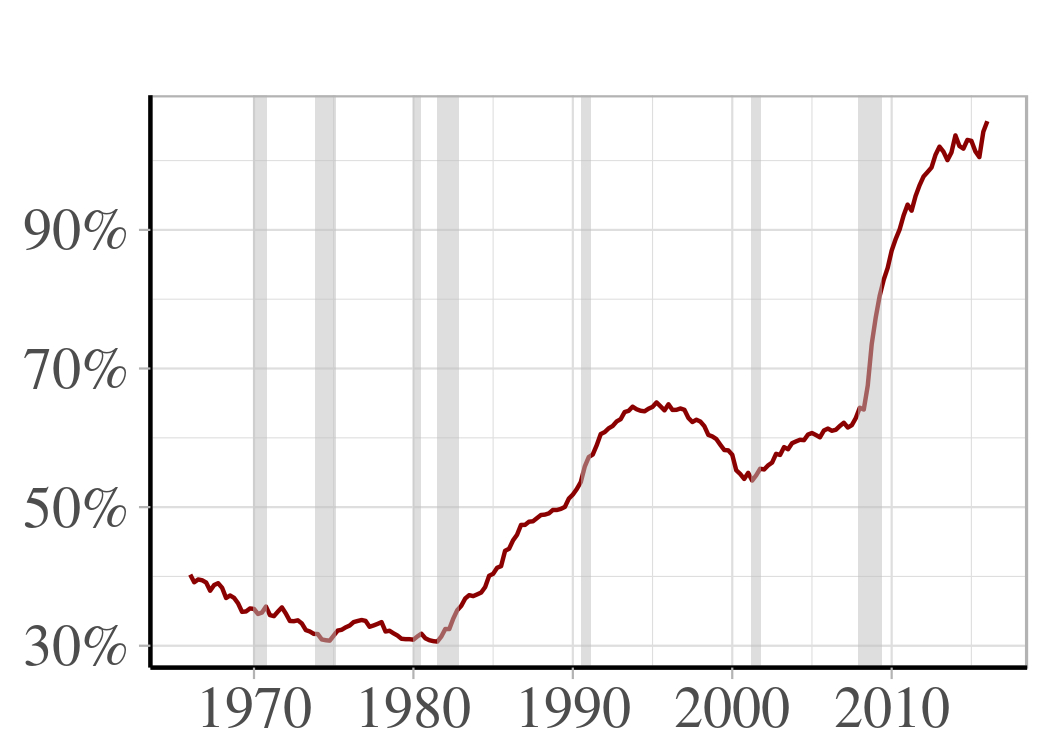
\includegraphics[width=\textwidth]{./plots/debt.png}
    \end{column}

    \begin{column}{0.5\textwidth}
      \ \ \ \ \ Federal Deficit
      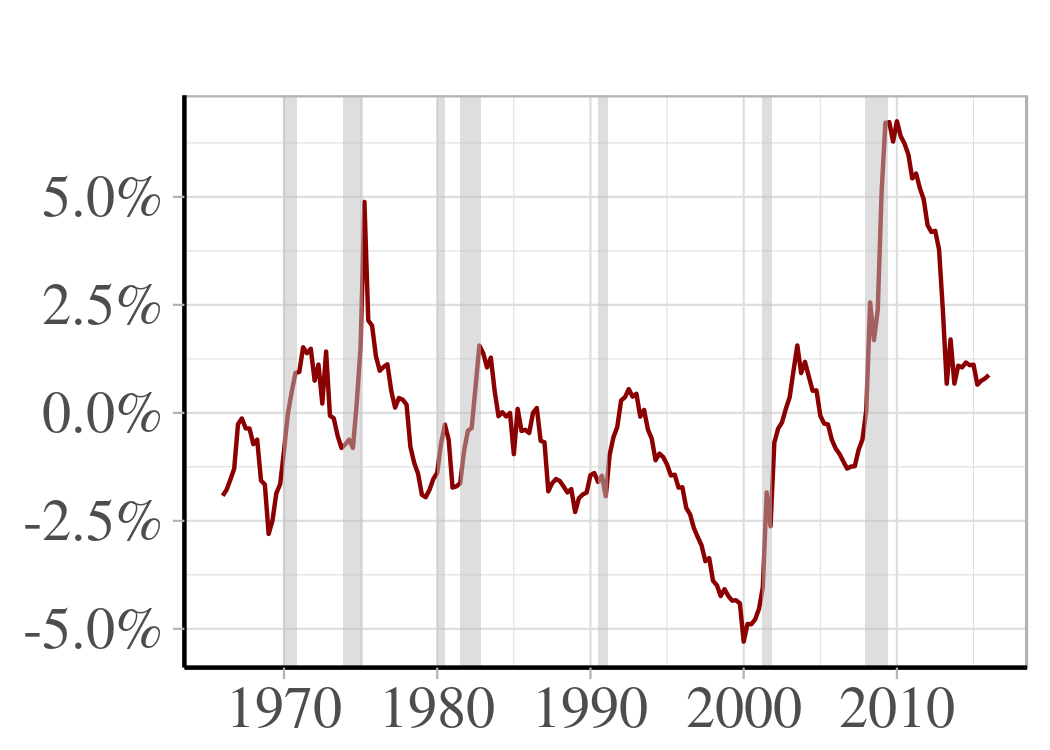
\includegraphics[width=\textwidth]{./plots/deficit.png}
    \end{column}
  \end{columns}
\end{frame}

\begin{frame}
  \ft{Fiscal Policy Variables}
  \uncover<+->{
  \begin{block}{Government Expenditures}
    \bi
    \item Federal government purchases of goods and services
    \item Macro target: Should \textit{decrease} as output gap \textit{increases}
    \item Debt target: Should \textit{decrease} as debt increases
    \ei
  \end{block}}

  \uncover<+->{
    \begin{block}{Transfers}
      \bi
      \item Payments made to individuals or on their behalf: unemployment benefits, college education subsidies, etc
      \item Macro target: Should \textit{decrease} as output gap \textit{increases}
      \item Debt target: Should \textit{decrease} as debt increases
    \ei
  \end{block}}

  \uncover<+->{
    \begin{block}{Taxes}
      \bi
      \item Federal revenue collected from all sources
      \item Macro target: Should \textit{increase} as output gap \textit{increases}
      \item Debt target: Should \textit{increase} as debt increases
    \ei
  \end{block}}

  
\end{frame}

\begin{frame}
  \ft{Fiscal Variables}
  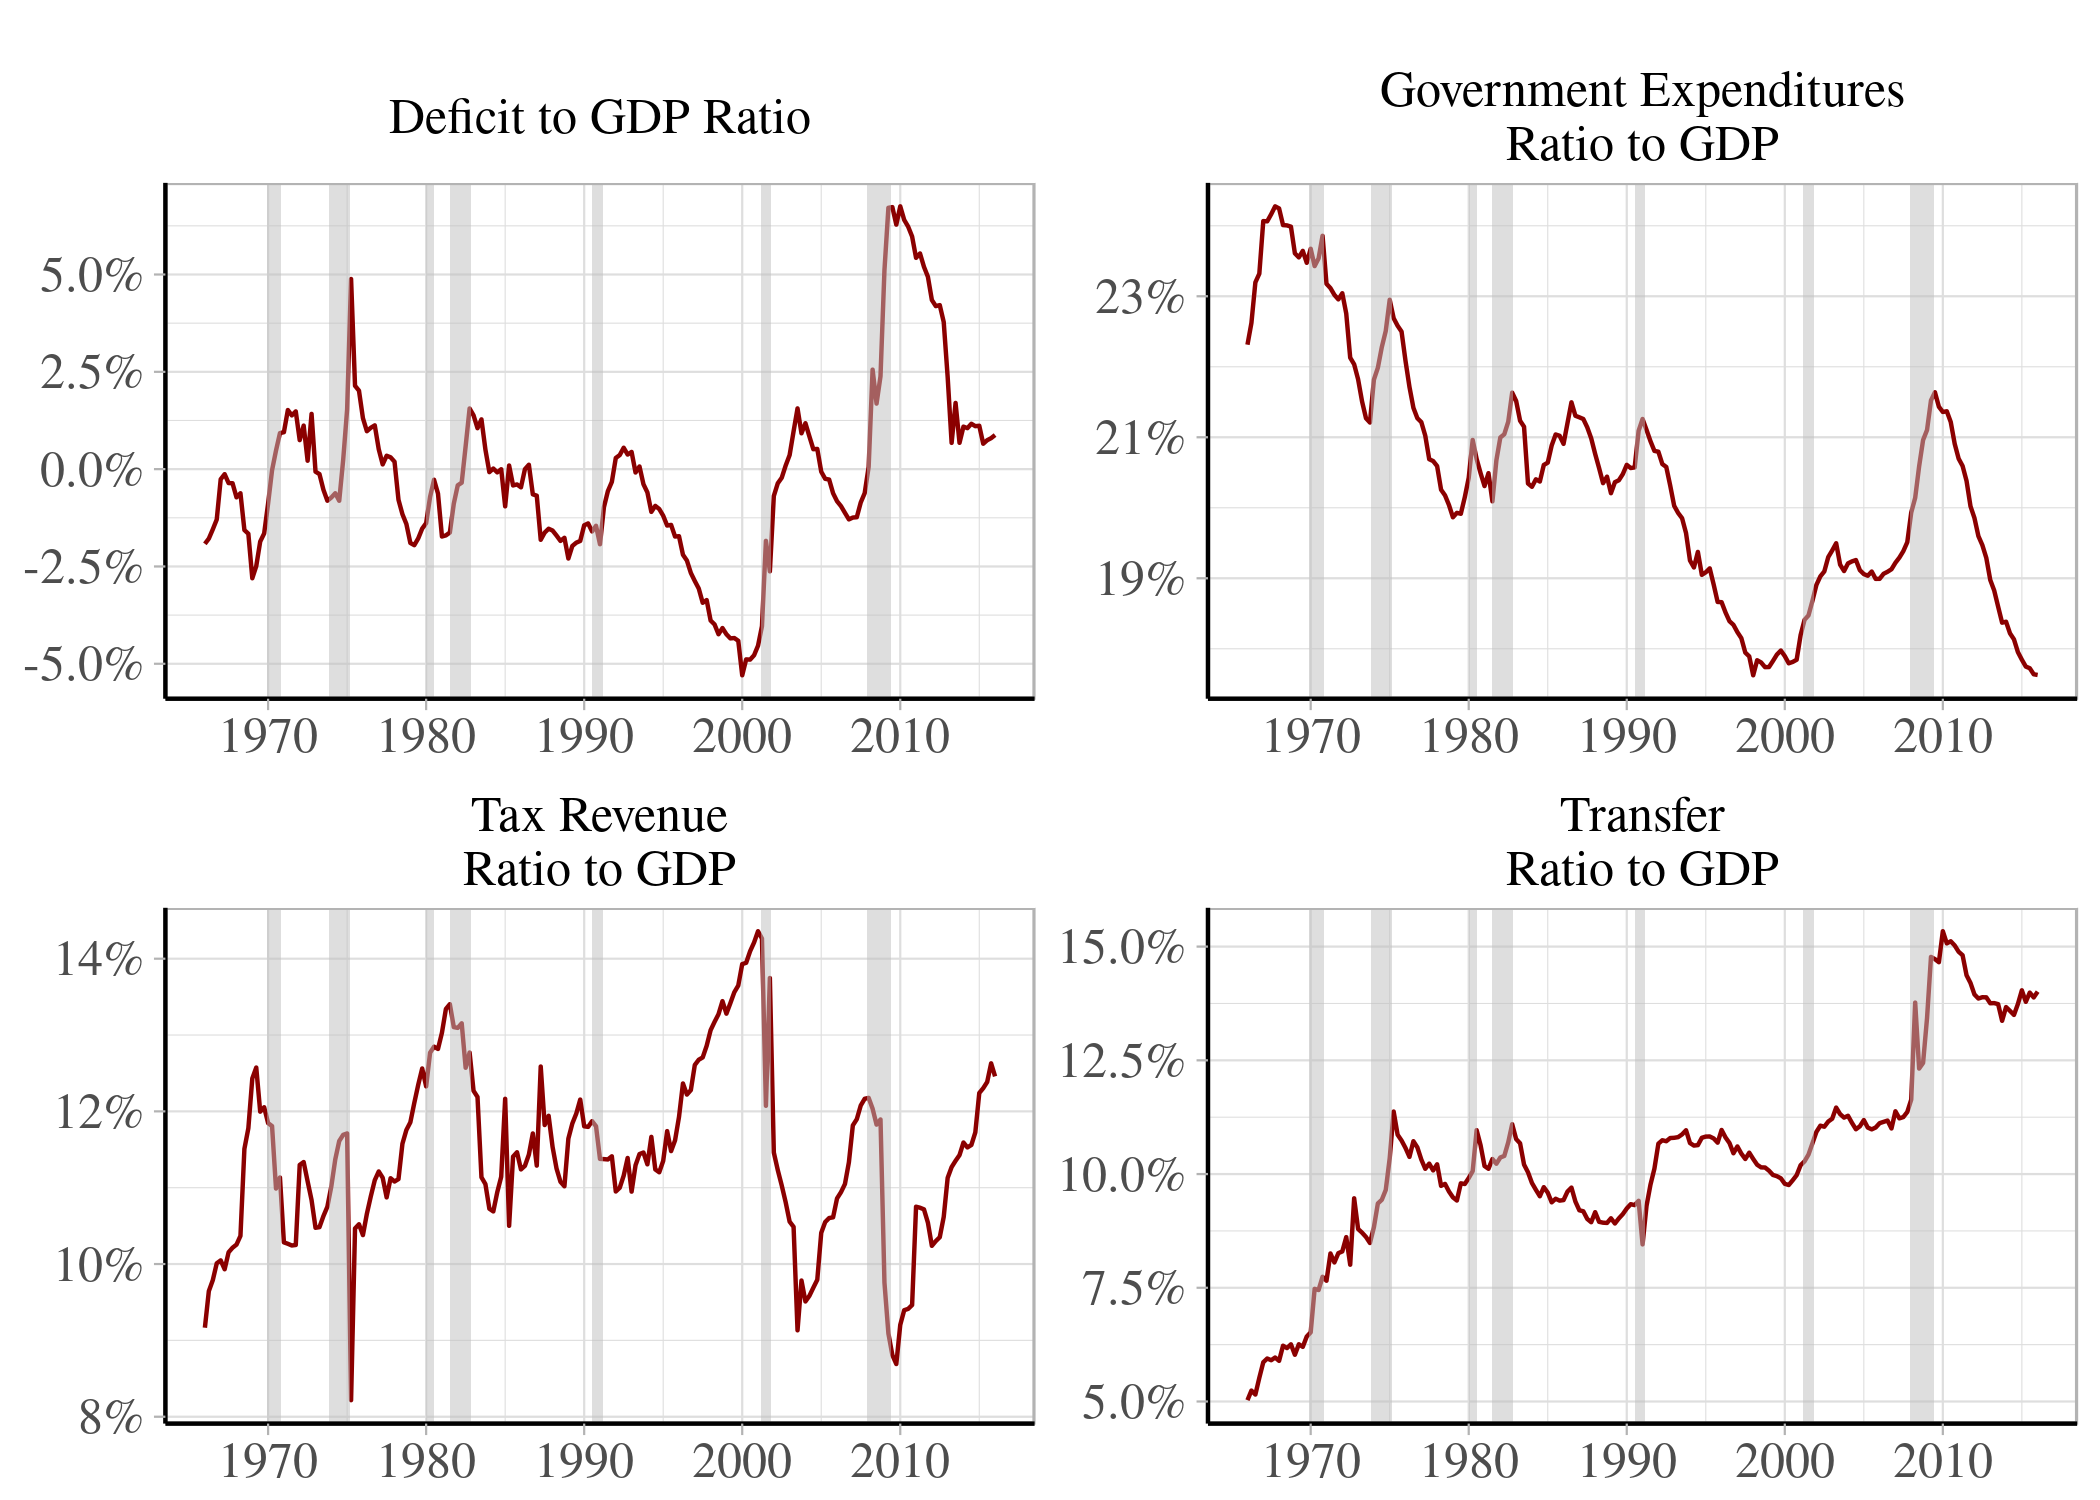
\includegraphics[align=t,width=0.95\textwidth]{./plots/data.png}
\end{frame}


\begin{frame}
  \ft{Purpose}
  \uncover<+->{
    \begin{block}{Investigate Evidence for Fiscal Policy Switching}
      \bi
      \item Which fiscal variables are important for economic stabilization?
      \item Which fiscal variables are important for servicing debt?
      \item Is there switching?
        \ei
    \end{block}
  }
  
  \uncover<+->{
  \begin{block}{Describe debt service}
    \begin{enumerate}
    \item How do fiscal policy variables respond to \textit{debt / GDP}?
    \item What is the implied target for \textit{debt / GDP}?
    \item Is there switching in these fiscal policy responses?
    \item Is there switching in the long-run debt target?
    \end{enumerate}
  \end{block}
  } % end uncover

  \uncover<+->{
  \begin{block}{Describe stabilizing behavior (macro targets)}
    \begin{enumerate}
    \item How do fiscal policy variables respond to \textit{output gap}?
    \item Is there switching in these fiscal policy responses?
    \end{enumerate}
  \end{block}
  } % end uncover
\end{frame}



\begin{frame}
  \ft{Three Sources for Regime Switching}
  \begin{footnotesize}
    \uncover<+->{\begin{block}{Long-run Debt Target Regimes}
    \setbeamertemplate{enumerate items}[default]
    \begin{enumerate}[{Regime} A:]
      \setcounter{enumi}{11}
      \item \textit{Low} long-run target for debt/GDP 
      \setcounter{enumi}{7}
      \item \textit{High} long-run target for debt/GDP 
    \end{enumerate}
  \end{block}}

  \uncover<+->{
    \begin{block}{Fiscal Financing}
      \bi
      \item Implied long-run targets (as \% of GDP) for
        \bi
        \item Government expenditures
        \item Transfers
        \item Taxes
        \ei
      \item Macroeconomic stabilization and debt-servicing behaviors for each
        \ei
        
      \setbeamertemplate{enumerate items}[default]
      \vspace*{-0.5pc}\begin{enumerate}[{Regime} A:]
      \item Fiscal behavior A
      \item Fiscal behavior B
      \end{enumerate}
    \end{block}
  }

  \uncover<+->{
    \begin{block}{Fiscal Volatility}
          \setbeamertemplate{enumerate items}[default]
          \begin{enumerate}[{Regime} A:]
        \setcounter{enumi}{18}
        \item \textit{Stable}, relatively smaller variances
        \setcounter{enumi}{21}
        \item \textit{Volatile}, relatively larger variances 
      \end{enumerate}
    \end{block}
  }
  \end{footnotesize}
  
\end{frame}

\begin{frame}
  \ft{Timing of Fiscal Regimes}
  \begin{center}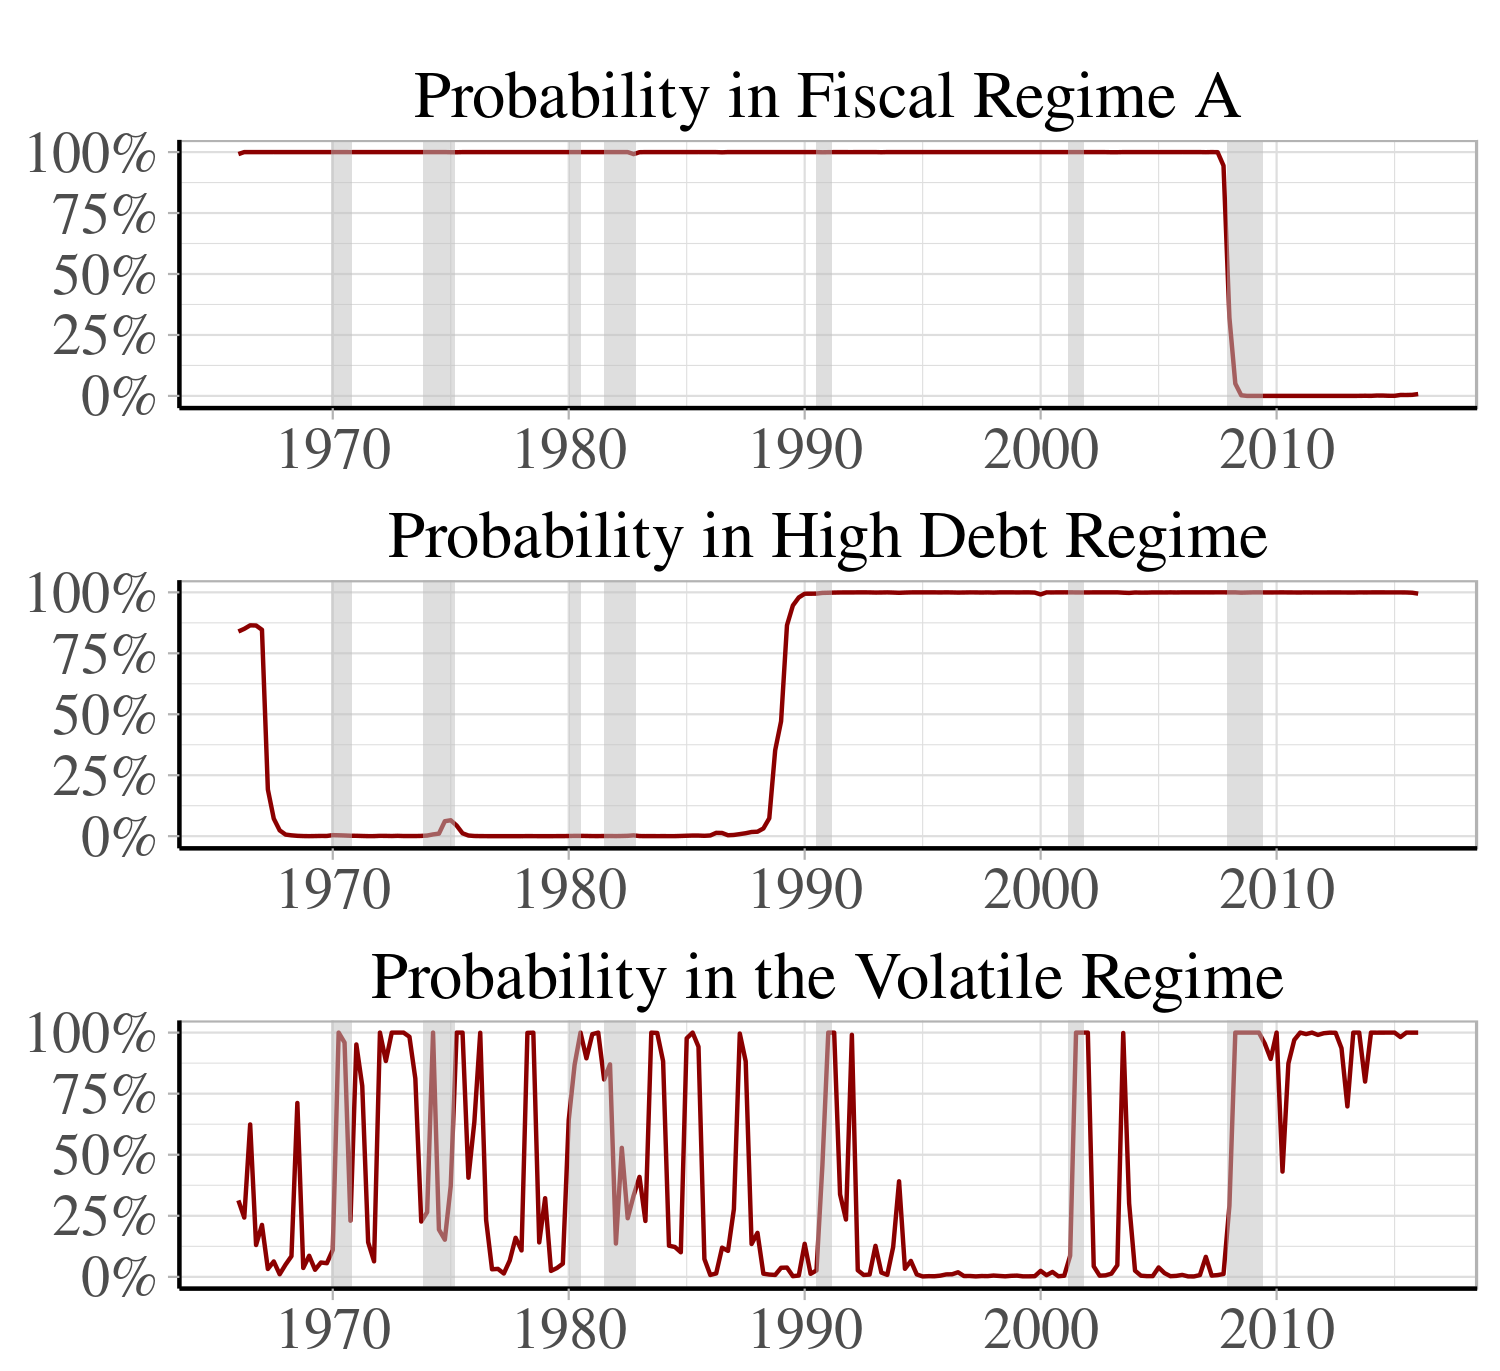
\includegraphics[align=t,height=0.85\textheight]{./plots/regimes.png}\end{center}
\end{frame}


\begin{frame}
  \ft{Results: Government Expenditures Behavior}
  \small{
    \uncover<+->{\begin{block}{Posterior Parameter Distributions Under Regimes A \& B}
      \setlength{\tabcolsep}{2pt}
      \begin{tabular}{clcccc}
        & & \multicolumn{2}{c}{Fiscal Regime A} & \multicolumn{2}{c}{Fiscal Regime B} \\ 
        Param. & Description & Median & 90\% Bounds & Median & 90\% Bounds \\ \hline
        \hl{2}{$\bar{g}$} & \hl{2}{Long-run gov target} & \hl{2}{0.19} & \hl{2}{(0.18, 0.20)} & \hl{2}{0.31} & \hl{2}{(0.29, 0.32)} \\ [0.2pc]
        \hl{3}{$\psi_{g}$} & \hl{3}{Resp to output gap} & \hl{3}{-0.32} & \hl{3}{(-0.38, -0.28)} & \hl{3}{-0.43} & \hl{3}{(-0.45, -0.39)} \\ [0.2pc]
        \hl{4}{$\gamma_{g}$} & \hl{4}{Resp to debt} & \hl{4}{-0.55} & \hl{4}{(-0.61, -0.49)} & \hl{4}{-0.44} & \hl{4}{(-0.50, -0.40)} \\ \hline
      \end{tabular}
    \end{block}}

    \uncover<+->{\begin{block}{Description}
      \bi
      \item<2> \hl{2}{Fiscal Regime A has \textbf{lower long-run} government expenditures}
      \item<3> \hl{3}{Fiscal regime A has gov exp \textbf{less responsive to output gap}}
      \item<4> \hl{4}{Fiscal regime A has gov exp \textbf{more responsive to debt}}
      \ei
    \end{block}
    }
  }
\end{frame}

\begin{frame}
  \ft{Results: Tax Behavior}
  \small{
    \uncover<+->{\begin{block}{Posterior Parameter Distributions Under Regimes A \& B}
      \setlength{\tabcolsep}{2pt}
      \begin{tabular}{clcccc}
        & & \multicolumn{2}{c}{Fiscal Regime A} & \multicolumn{2}{c}{Fiscal Regime B} \\ 
        Param. & Description & Median & 90\% Bounds & Median & 90\% Bounds \\ \hline
        \hl{2}{$\bar{\tau}$} & \hl{2}{Long-run tax target} & \hl{2}{0.14} & \hl{2}{(0.13, 0.14)} & \hl{2}{0.28} & \hl{2}{(0.25, 0.29)} \\ [0.2pc]
        \hl{3}{$\psi_{\tau}$} & \hl{3}{Resp to output gap} & \hl{3}{0.69} & \hl{3}{(0.68, 0.72)} & \hl{3}{0.47} & \hl{3}{(0.44, 0.55)} \\ [0.2pc]
        \hl{4}{$\gamma_{\tau}$} & \hl{4}{Resp to debt} & \hl{4}{0.25} & \hl{4}{(0.23, 0.29)} & \hl{4}{0.34} & \hl{4}{(0.26, 0.44)} \\ \hline
      \end{tabular}
    \end{block}}

    \uncover<+->{\begin{block}{Description}
      \bi
      \item<2> \hl{2}{Fiscal Regime A has \textbf{lower long-run} tax target}
      \item<3> \hl{3}{Fiscal regime A has taxes \textbf{more responsive to output gap}}
      \item<4> \hl{4}{Fiscal regime A has taxes \textbf{less responsive to debt}}
      \ei
    \end{block}
    }
  }
\end{frame}


\begin{frame}
  \ft{Results: Transfers Behavior}
  \small{
    \uncover<+->{\begin{block}{Posterior Parameter Distributions Under Regimes A \& B}
      \setlength{\tabcolsep}{2pt}
      \begin{tabular}{clcccc}
        & & \multicolumn{2}{c}{Fiscal Regime A} & \multicolumn{2}{c}{Fiscal Regime B} \\ 
        Param. & Description & Median & 90\% Bounds & Median & 90\% Bounds \\ \hline
        \hl{2}{$\bar{n}$} & \hl{2}{Long-run transfers} & \hl{2}{0.11} & \hl{2}{(0.10, 0.13)} & \hl{2}{0.18} & \hl{2}{(0.17, 0.20)} \\ [0.2pc]
        \hl{3}{$\psi_{n}$} & \hl{3}{Resp to output gap} & \hl{3}{-0.46} & \hl{3}{(-0.49, -0.41)} & \hl{3}{-0.50} & \hl{3}{(-0.54, -0.43)} \\ [0.2pc]
        \hl{4}{$\gamma_{n}$} & \hl{4}{Resp to debt} & \hl{4}{-0.33} & \hl{4}{(-0.37, -0.26)} & \hl{4}{-0.51} & \hl{4}{(-0.55, -0.47)} \\ \hline
      \end{tabular}
    \end{block}}

    \uncover<+->{\begin{block}{Description}
      \bi
      \item<2> \hl{2}{Fiscal Regime A has \textbf{lower long-run} transfers}
      \item<3> \hl{3}{Regimes are \textbf{not different on responsiveness to output gap}}
      \item<4> \hl{4}{Fiscal regime A has transfers \textbf{less responsive to debt}}
      \ei
    \end{block}
    }
  }
\end{frame}



\begin{frame}
  \ft{Results: Debt Regimes}
  \small{
    \uncover<+->{\begin{block}{Posterior Parameter Distributions Under Low \& High Debt Regimes}
      \setlength{\tabcolsep}{2pt}
      \begin{tabular}{clcccc}
        & & \multicolumn{2}{c}{Low Debt Regime} & \multicolumn{2}{c}{High Debt Regime} \\ 
        Param. & Description & Median & 90\% Bounds & Median & 90\% Bounds \\ \hline
        $\bar{b}$ & Debt/GDP target & 0.37 & (0.34, 0.39) & 0.60 & (0.55, 0.64) \\ \hline
      \end{tabular}
    \end{block}}

    \uncover<.->{\begin{block}{Debt Regimes}
      Low debt regime $\approx$ 37\% of GDP\\
      High debt regime $\approx$ 60\% of GDP
    \end{block}
    }
  }
\end{frame}

\begin{frame}
  \ft{Results: Volatility Regimes}
  \small{
    \uncover<+->{\begin{block}{Posterior Parameter Distributions Under Stable and Volatile Regimes}
       \setlength{\tabcolsep}{4pt}
       \begin{tabular}{clcccc}
        & & \multicolumn{2}{c}{Stable Regime} & \multicolumn{2}{c}{Volatile Regime} \\ 
        Param. & Description & Median & 90\% Bounds & Median & 90\% Bounds \\ \hline
        $\sigma_{g}$ & Gov stdev & 0.10 & (0.09, 0.11) & 0.19 & (0.17, 0.22) \\ 
        $\sigma_{\tau}$ & Tax stdev & 0.10 & (0.10, 0.11) & 0.29 & (0.28, 0.30) \\ 
        $\sigma_{n}$ & Transfers stdev & 0.06 & (0.06, 0.08) & 0.22 & (0.19, 0.26) \\ 
        $\sigma_{d}$ & Deficit stdev & 0.08 & (0.08, 0.10) & 0.20 & (0.19, 0.22) \\ \hline
      \end{tabular}
    \end{block}}
  }
  \ \\
  \textcolor{BrickRed}{All standard deviations are larger in volatile regime,\\\textbf{most more than double}.}
\end{frame}



\begin{frame}
  \ft{Conclusions}
  \bi
  \item<+-> Evidence of switching in all three dimensions.
  \item<+-> Switch from low-debt to high-debt regime in 1989.
  \item<+-> Single, permanent, switch in fiscal policy behavior in 2008.
    \bi
    \item Government expenditures playing larger role in macroeconomic stabilization, smaller role in balancing budget.
    \item Taxes play smaller role in macroeconomic stabilization, larger role in balancing budget.
      \ei
  \item<+-> Many switches from stable to volatile fiscal regimes, usually around and following recessions.
  \ei   
\end{frame}


\end{document}

